\section{Meilenstein 1: Die Anwendungsschicht}

Der erste Meilenstein umfasste das Anwendungsgrundgerüst, in welches das spätere Spiel eingebettet werden sollte.
Zu diesem Zeitpunkt war es aufgrund vorhandener Erfahrung im Bereich Frontend- und UI-Entwicklung generisch implementiert, bekannte Entwurfsmuster und Paradigmen aus dem Objektorientierten Design (im Folgenden OOD) wurden umgesetzt.
Ziel war es, ein robustes Fenstermanagement auf Basis von \textit{glfw}~\cite{glfwHomepage} zu implementieren, um den Fokus der nachfolgenden Meilensteine auf die Einbindung der Spielsysteme und -mechaniken zu legen.
In diesem Meilenstein wurde außerdem die Abstraktion der Rendering-Engine eingeführt, aus dem eine Spezialisierung zur Anbindung an ein \textit{OpenGL}-Backend~\cite{OpenGLHomepage} entwuchs.\\

In dieser frühen Phase wurden Designentscheidungen getroffen, die in den in späteren Meilensteinen entstandenen tieferen Schichten so nicht mehr zu finden sind.
Insbesondere der stark objektorientierte Ansatz wurde mit zunehmenden Verständnis der Anforderungen leistungsfähiger Spiele-Engines zugunsten eines \textit{Composition over Inheritance}-Ansatzes~\cite[S. 20]{GHJV94} verworfen, der in Meilenstein 5 in einer ECS-Architektur mündete (siehe Abschnitt~\ref{sec:meilenstein_5}).\\


\begin{figure}
    \centering
    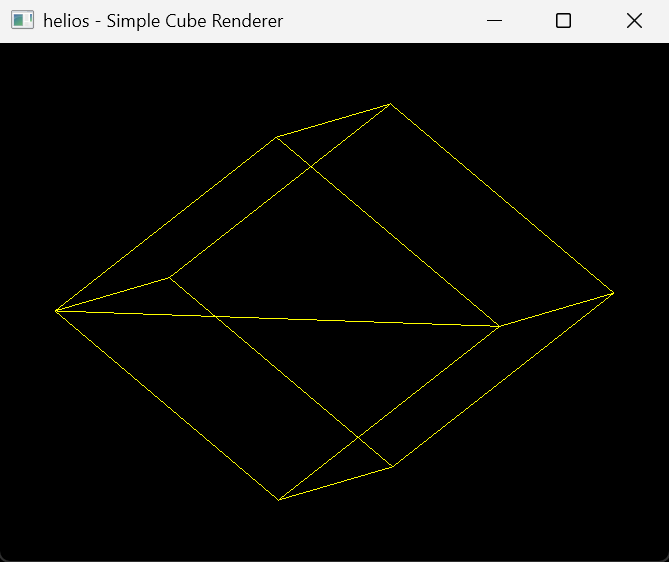
\includegraphics[width=0.4\columnwidth]{content/de/iterative evolution/img/simplecuberendering}
    \caption{Screenshot der ersten lauffähigen Anwendung mit der helios Engine, der \textit{Simple Cube Rendering Demo}, die einen rotierenden Würfel darstellt.
    Die zugrundeliegende Architektur implementiert bereits wesentliche Komponenten der Anwendungsschicht, darunter das Fenstermanagement sowie ein Event-System nach dem \textit{Publish-Subscribe}-Entwurfsmuster. (Quelle: eigene Aufnahme)}
    \label{fig:simplecuberendering}
\end{figure}

Im Zuge der Entwicklung der tiefer liegenden Schichten musste die Anwendungsschicht nur geringfügig angepasst werden, größere Änderungen ergaben sich hauptsächlich durch die Umstrukturierung von Modulen.
Signifikante Änderungen hinsichtlich der Funktionalität betrafen die Handhabung von Viewports, worauf wir im nächsten Abschnitt eingehen.